\chapter{Experiment} \label{ch:experiment}

We obtained the dataset of spoken digits, 15 utterances for each person per digit, and 3 persons in total. The recordings were done in moderately quiet environments using a general-purpose microphone.

For the obtained dataset, the trimming algorithm presented exceptionally accurate results. The results were close to 88\% for the error of speech signal's endpoints missing by 100ms.

\begin{figure}
    \centering
    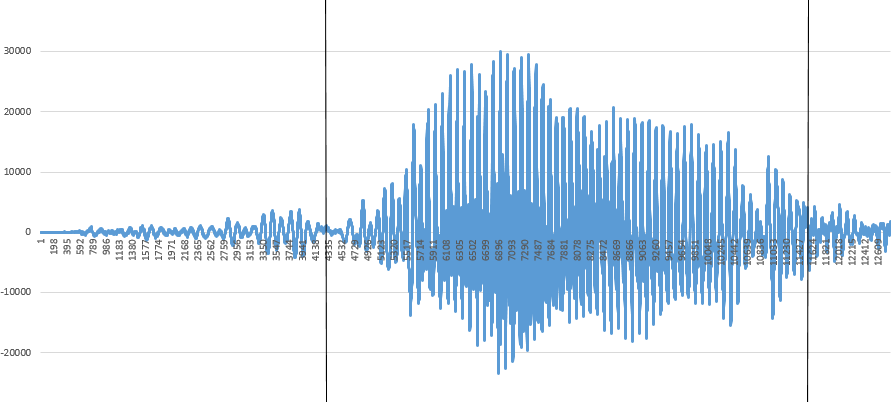
\includegraphics[scale=0.7]{nine-trim}
    \label{fig:nine-trim}
    \caption{Automatic trimming of Nine}
\end{figure}

\begin{minipage}{0.6\textwidth}
    \begin{figure}[H]
        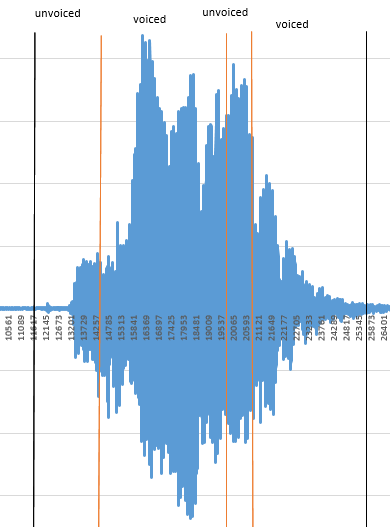
\includegraphics[scale=0.9]{zero-phoneme-segmentation}
        \caption{Phoneme segmentation of Zero}
        \label{fig:zero-phoneme-segementation}
    \end{figure}
    \end{minipage} \hfill
    \begin{minipage}{0.5\textwidth}
        The figure \ref{fig:zero-phoneme-segementation} shows the utterance of zero in which phoneme segmentation gives good result. For many other utterances, our implementation gave erratic results. The problem was seen to be an improper choice of voiced/unvoiced threshold, hence there were few small unvoiced segments between long stretches of voiced segments. This behaviour caused a major decrease (from 77\% down to 69\%) in the accuracy of the system as can be seen by the tables below.
        We also notice that due to the calculation of autocorrelation function, phoneme segmentation was approximately a ~5 second operation for each utterance. This would make it unsatisfactory for real-time use.
\end{minipage}

\begin{center}
\begin{table}[]
    \centering
    \begin{tabular}{@{}lllllllllll@{}}
    \cmidrule(l){2-11}
    Digit    & 0  & 1  & 2  & 3  & 4  & 5  & 6  & 7  & 8  & 9  \\ \cmidrule(l){2-11} 
    Accuracy & 62 & 80 & 86 & 64 & 95 & 77 & 73 & 73 & 86 & 82 \\ \cmidrule(l){2-11} 
    \end{tabular}
    \caption{Accuracy without using phoneme segmentation}
    \end{table}
\end{center}
\begin{table}[]
    \centering
    \begin{tabular}{@{}lllllllllll@{}}
    \cmidrule(l){2-11}
    Digit    & 0  & 1  & 2  & 3  & 4  & 5  & 6  & 7  & 8  & 9  \\ \cmidrule(l){2-11} 
    Accuracy & 73 & 46 & 66 & 73 & 66 & 80 & 53 & 80 & 86 & 66 \\ \cmidrule(l){2-11} 
    \end{tabular}
    \caption{Accuracy with using phoneme segmentation}
    \end{table}
            